\chapter{Grundlagen}
\label{cha:Grundlagen}
Im folgenden Kapitel sollen die zum Verständnis der Arbeit nötigen Grundlagen erläutert werden. Anfangs werden die elektrochemischen Grundlagen der Elektrolyse von Wasser vorgestellt sowie deren thermodynamische Zusammenhänge geschildert. Zudem wird die ideale Zellspannung hergeleitet und es werden wesentliche Verlustmechanismen benannt. Weiterhin werden gängigen technischen Lösungen der Wasserelektrolyse vorgestellt. Im Anschluss werden Gemeinsamkeiten und Unterschiede von Elektrolyseuren und Brennstoffzellen dargelegt. \\


\section{Elektrolyse}
\label{sec:Elektrolyse}
Als Elektrolyse bezeichnet man einen chemischen Prozess, bei dem eine Redoxreaktion durch elektrische Spannung erzwungen wird. 
Um eine kontrollierbare Durchführung der Reaktion sicherzustellen, muss eine räumliche und elektrische Trennung der Oxidation und Reduktion vorliegen \cite{Tjaarks}. Allerdings muss Ionenaustausch zwischen Anode und Kathode möglich sein und dies wird durch ein Elektrolyt erreicht.

\subsection{Wasserelektrolyse}
\label{subsec:Elektrolyse} 
Bei der Wasserelektrolyse wird dieses Prinzip angewendet, um aus Wassermolekülen elementaren Wasserstoff und elementaren Sauerstoff zu gewinnen. Dabei liegt folgende allgemeine Reaktionsgleichung vor:   
\begin{align}
	\ce{ H2O &-> H2 + 1/2O2}
\end{align}
Die allgemeine Reaktionsgleichung ist dabei unabhängig vom Elektrolyt, wohingegen sich die Oxidations- und Reduktionsgleichungen unterscheiden. Die Oxidation findet an der Anode statt und hat Sauerstoff als Produkt. An der Kathode wird durch die Reduktion Wasserstoff gebildet. Es gibt drei mögliche Ladungsträger bei der Wasserelektrolyse: Hydroxidionen, Protonen oder Oxidionen. Zu den verschiedenen Ladungsträgern werden im Abschnitt !!!!!!!!!!!!! technische Verfahren angeführt und erläutert.
\begin{figure}[h]
	\centering
		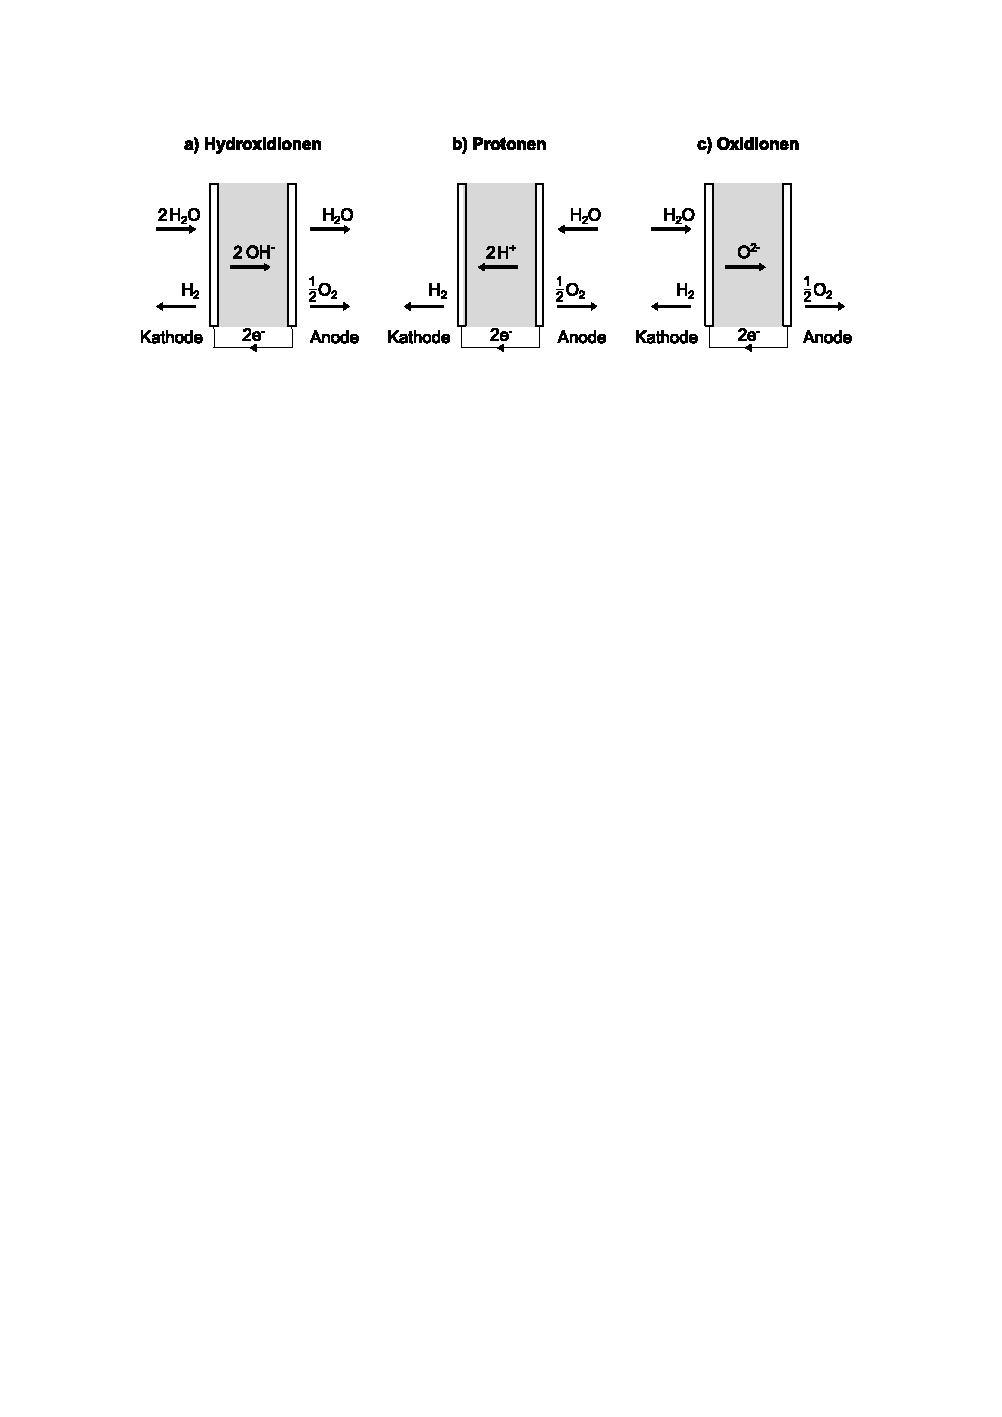
\includegraphics[scale=1]{Figures/LadungstraegerBeiDerWasserelektrolyse}
		\caption{Ladungsträger bei der 
		Wasserelektrolyse [\cite{ISBN 978-3-95806-217-7}]}
\label{fig:LadungstraegerBeiDerWasserelektrolyse}	
\end{figure}

\subsection{Thermodynamische Betrachtung}
\label{subsec:Energetische Betrachtung der Wasserelektrolyse}
Die benötigte Energie bei einer Redoxreaktion entspricht der Reaktionsenthalpie $\Delta H_R$ und lässt sich aus den Bildungsenthalpien ($\Delta_f H_i$) und stöchometrischen Koeffizienten ($\nu_i$) der Edukte und Produkte bestimmen:
\begin{align}
 	\Delta H_R = \sum{\nu_i \Delta_f H_i}
\end{align}
Unter der Annahme, dass die nötige thermische Energie vorliegt, entspricht die zur Reaktion benötigte elektrische Energie  der freien Reaktionsenthalpie $\Delta G_R$, welche sich über die Reaktionsentropie $\Delta S_R$ errechnen lässt.
\begin{align}
	\Delta G_R = \Delta H_R - T\Delta S_R \\
 	\Delta S_R = \sum{\nu_i S_i}
\end{align}

Für die Wasserstoffelektrolyse (3.1) bei Standardtbedingungen ($T_0 = \SI{298,15}{\kelvin}$ und $p_0 = \SI{101,325}{\kilo\pascal}$) ergibt sich mit den Daten aus Tabelle 3.1 die Reaktionsenthalpie zu $\Delta H^0_R = \SI{285,25}{\kilo\J\per\mol}$ und die freie Enthalpie zu $\Delta G^0_R = \SI{236,59}{\kilo\J\per\mol}$. 
\begin{table}[ht]
		\centering
		\caption{Standardtbildungsenthalpien und Standardtentropien für $\SI{298,15}{\kelvin}$ [\cite{?%Entwicklung und Charakterisierung von Elektroden für die Sauerstoffentwicklung in der alkalischen Wasserelektrolyse
		}] sowie stöchometrische Koeffizienten aus (3.1)}
		\begin{tabular}{c c c c}
		\toprule
		\multirow{2}{*}{Komponenten i} & 
		\multicolumn{1}{c}{$\Delta_f H^0_i$} & 
		\multicolumn{1}{c}{$S^0_i$} &
		\multicolumn{1}{c}{$\nu_i$}
		\\
		& 
		\multicolumn{1}{c}{$\textrm{[kJ/mol]}$}& 
		\multicolumn{1}{c}{$\textrm{[J/(molK)]}$} &
		\multicolumn{1}{c}{$\textrm{[--]}$}
		\\
		\midrule
		$\ce{H2O}$ & -285,25 & 70,12 & -1\\
		$\ce{O2}$ & 0 & 205,25 & 1\\
		$\ce{H2}$ & 0 & 130,7 & $\textrm{1/2}$\\
		\bottomrule
		\end{tabular}
		\label{tab:rule}
		\end{table}	
			
\subsection{Reversible Zellspannung}
\label{subsubsec:Zellspannung}
Mit der Faraday Konstante ($F=\SI{96485,3}{\coulomb\per\mol}$) und der Anzahl der pro Reaktion transferierten Elektronen ($n = 2$) lässt sich die thermoneutrale Spannung bei Standardtbedingungen $U^0_{th}$ sowie die reversible Zellspannung bei Standardbedingungen $U^0_{rev}$ errechnen:
\begin{align}
 U^0_{th} = \frac{\Delta H^0_R}{nF} = \SI{1,478}{\volt}\\
 U^0_{rev} = \frac{\Delta G^0_R}{nF} = \SI{1,226}{\volt}
\end{align}

!!!!!!Über die Nernst-Gleichung lässt sich die Abhängigkeit der reversiblen Zellspannung $U_{rev}$ von der Temperatur und den Partialdrücken der Produkte ($p_{H_2}$ für Wasserstoff und $p_{O_2}$ für Sauerstoff) sowie der Aktivität des Wassers ($a_{H_{2}O}$) beschreiben (zitat!!!). Im Falle der Festoxid Elektrolyse muss, weil gasförmiges Wasser vorliegt, der Partialdruck des Wassers ($a_{H_{2}O}$) verwendet werden.
\begin{align}
 U_{rev} =  U^0_{rev} + \frac{RT}{nF}\ln{(\frac{p_{H_2}\sqrt{p_{O_2}}}{a_{H_{2}O}})} \\
 U_{rev} =  U^0_{rev} + \frac{RT}{nF}\ln{(\frac{p_{H_2}\sqrt{p_{O_2}}}{p_{H_{2}O}})}
\end{align}

\subsection{Überspannungen}
\label{subsubsec:Überspannungen}
Die reale Zell-Spannung $U_{real}$ ist im Betrieb aufgrund von Verlusten immer größer als die reversiblen Zellspannung. Die maßgeblichen Verluste, auch Überspannungen genannt, werden üblicherweise in drei Bereiche aufgeteilt: Aktivierungsverluste ($U_{Akt}$), Ohmsche Verluste ($U_{Ohm}$) und Konzentrationsüberspannung ($U_{Diff}$)\cite{guideline}. Ein weiteres Phänomen sind Diffusionsströme von Wasserstoff auf die Anodenseite und von Sauerstoff auf die Kathodenseite, allerdings ist deren Größenordnung aus Sicherheitsaspekten gering zuhalten, was in !!!!!! näher erläutert wird. Daher werden Diffusionsströme in dieser Arbeit als vernachlässigbar klein angenommen. 
\begin{align}
 U_{real} =  U_{rev} + U_{Akt} + U_{Ohm} + U_{Diff}
\end{align}   
\paragraph{Aktivierungsverluste} \ \\
Aktivierungsverluste kommen durch die elektrochemischen Vorgänge an den Oberflächen er Elektroden und ihrer Kinetik zustande. Dabei treten zwei Phänomene auf:  Einerseits chemische (wegen des chemischen Gleichgewichtszustands der Ionen an der Grenzfläche zwischen Elektrode und Elektrolyt) und andererseits elektrische (aufgrund des Ladungstransports durch das elektrische Feld an der Grenzfläche)\cite{Solid Oxide Electrolyzer Cell Modeling: A Review}.\\

\paragraph{Ohmsche Verluste} \ \\
Ohmsche Verluste werden durch elektrische sowie ionische Widerstände und Kontaktwiderständen zwischen den Komponenten verursacht. Ionischen Widerstände, welche sich in der Membran (bei alkalischer und PEM-Elektrolyse) und an den Elektrodenoberflächen lokalisieren lassen, dominieren üblicherweise die Ohmschen Verluste \cite{Solid Oxide Electrolyzer Cell Modeling: A Review}. Elektrisch Widerstände treten in den Elektroden und an der Kontaktierung der Zelle auf und lassen sich somit durch den Aufbau der Zelle beeinflussen \cite{ISBN 978-3-95806-217-7}.\\

\paragraph{Diffusionsüberspannungen}\ \\
Diffusionsüberspannungen treten auf, wenn aufgrund hoher Stromdichten, eine Überpopulation von Produktgasen an den Elektroden entsteht. Die Gase bilden dann Bläschen auf den Elektrodenoberflächen und behindern somit die Elektrolyse der Wassermoleküle. Diffusionsüberspannungen treten verstärkt bei hohen Stromdichten auf und sind somit ein limitierender Faktor für die maximale Stromdichte eines Elektrolyseurs [\cite{A semiempirical study of the temperature dependence
of the anode charge transfer coefficient of a 6 kW PEM
electrolyzer}].\\

\subsection{Alkalischer Elektrolyseur}
\label{subsec:Alkalischer Elektrolyseur}
Die alkalische Elektrolyse ist eine ausgereifte Technik und der derzeitige Standard für groß dimensionierte Elektrolyseure. Anlagen mit einer Leistung Wasserstoffproduktion von bis zu \SI{130}{\mega\W} [\cite{
%https://doi.org/10.1007/978-3-319-72459-1
}] sind derzeit im Betrieb und die minimale Teillast liegt nach \cite{
%G. Guandalini, S. Campanari, G. Valenti, Comparative assessment and safety issues in state-of-the-art hydrogen production technologies. Int. J. Hydrogen Energy, 41, 18901–18920 (2016)
} bei ungefähr 20\%. Als Elektrolyt dient üblicherweise Kalilauge, deren Konzentration zwischen 25 und 30\% liegt. Grund dafür ist, das der Base-Gehalt der Lösung maßgeblich deren Leitfähigkeit beeinflusst. Als Ladungsträger in der Lösung fungieren Hydroxidionen. Es werden metallische Elektroden verwendet, welche gelegentlich zur Steigerung der Aktivität mit Edelmetallen beschichtet werden. Folgende Reaktionen laufen an der Kathode und Anode ab:
\begin{align}
  \ce{	&{Kathode:} &2H2O + 2 e^- &-> H2 + 2OH^-\\
  		&{Anode:} &2OH^- &-> H2O + O2 + 2 e^-} 
\end{align}
Um die produzierten Gase von einander getrennt zu halten, wird zwischen Anode und Kathode ein Diaphragma positioniert. Dies hat Performance aber auch Sicherheitsgründe, da elementarer Wasserstoff hochentzündlich ist. Aus diesem Grund sind alkalische Elektrolyseure auch in ihrer Dynamik eingeschränkt: Bevor das System abgeschaltet werden kann, müssen die Gasleitungen mit Inertgas gefüllt werden, um die Bildung einer explosiven Wasserstoff-Sauerstoff Mischung zu verhindern. Dies hat auch einen Einfluss auf den Anlaufvorgang des Systems, da die Gasqualität durch die anfangs vorliegenden Inertgase vermindert wird. 
Ein weiterer Nachteil aktueller technischer Anlagen der alkalischen Elektrolyse ist, das die maximale Stromdichte verglichen mit anderen Elektrolyseuren niedrig ausfällt [\cite{L. Bertuccioli, A. Chan, D. Hart, F. Lehner, B. Madden, E. Standen, Study on development of water electrolysis in the EU. Fuel Cells and Hydrogen Joint Undertaking (2014)}] gibt Stromdichten von $0,2-\SI{0,5}{\A\per\cm\squared}$ an.

\subsection{Protonen Austausch Membran (PEM) Elektrolyseur}
\label{subsec:Protonen Austausch Membran (PEM) Elektrolyseur}
PEM-Elektrolyseure werden seid 1950 entwickelt und derzeit im $\SI{1}{\mega\W}$ Bereich vertrieben. Ein Vorteile der Technologie sind die hohen erreichbaren Stromdichten von bis zu $\SI{0,5}{\A\per\cm\squared}$. Zudem können PEM-Elektrolyseure sehr dynamisch betrieben werden und ein Betrieb bei bis zu 10\% minimaler Teillast ist möglich [\cite{
%https://doi.org/10.1007/978-3-319-72459-1
}].\\
Als Ladungsträger fungieren Protonen und als Elektrolyt dient eine in destilliertem Wasser positionierte Protonen-Austausch-Membran (\textbf{P}roton \textbf{E}xchange \textbf{M}embran). Dies vereinfacht den Betrieb verglichen mit den mit stark basischer Lösung befüllten, alkalischen Elektrolyseuren erheblich. Die Protonenleitfähigkeit der Polymer-Membran wird durch Sulfonsäure-bindende Seitengruppen, sogenannte Idomere, erreicht \cite{ISBN 978-3-95806-217-7}.  Für die Dicke der Membran muss dabei ein Kompromiss zwischen Langlebigkeit und Durchlässigkeit gefunden werden \cite{review on PEM electrolyzer modelling: Guidelines for beginners}. Die Säure des Elektrolyts, so wie das Erstreben hoher Reaktionsgeschwindigkeiten führt zu hohen Kosten bei den Elektrodenmaterialien: Die Kathode besteht meist aus mit Platin beschichtetem Kohlenstoff, als Anode werden häufig als Oxid vorliegendes Irdium oder Ruthenium verwendet. Folgende Reaktionen laufen an der Kathode und Anode ab:
\begin{align}
  \ce{	&{Kathode:} &2H^+ + 2e^- &-> H2\\
  		&{Anode:} &H2O  &->  1/2O2 + 2H^+ + 2 e^-}
\end{align}
  		
\subsection{Feststoffoxid Elektrolyseur}
\label{subsec:Feststoffoxid Elektrolyseur}
Feststoffoxid(SO) Elektrolyseure sind seid 1980 in Entwicklung [\cite{
%A. Isenberg, Energy conversion via solid oxide electrolyte electrochemical cells at high temperatures. Solid State Ionics 3–4, 431–437 (1981)
}]. Sie haben aus thermodynamischer Sicht den Vorteil, dass sie Temperaturen von $600-\SI{900}{\degreeCelsius}$ betrieben werden. Somit wird bei der SOC-Elektrolyse dampfförmiges Wasser zerlegt, wohingegen bei alkalischen und PEM-Elektrolyseuren flüssiges Wasser vorliegt. Daraus resultiert, dass die zur Elektrolyse des Wassers benötigt Zellspannung und somit auch die zugeführte Elektrische Energie niedriger ausfällt. Dieser Effekt wird dadurch verstärkt, dass bei hohen Temperaturen die ohmschen Verluste sinken, wodurch niedrigere Überspannungen entstehen (\cite{https://doi.org/10.1007/978-3-319-72459-1}). Zudem steigt mit der Temperatur auch die Reaktionsgeschwindigkeit, weshalb keine teuren Katalysatormaterialien verwendet werden müssen [\cite{Performance and degradation of an SOEC stack with different cell
components}].\\
Ein Nachteil der gesteigerten Betriebstemperatur sind die höheren Ansprüche an die Temperaturbeständigkeit der Elektroden und des Elektrolyts. Als Elektrolyt wird meist Zirconiumdioxid ($\ce{ZrO2}$) verwendet, welches zur Steigerung Leitfähigkeit mit ungefähr $\SI{8}{\mol\%}$ Yttriumoxid ($\ce{Y2O3}$) stabilisiert wird (\cite{
Decomposition of 8.5 mol.% Y2O3-doped zirconia and its contribution to the degradation of ionic conductivity
}).
Das Elektrolyt wird zwischen zwei porösen Elektroden (Beispielsweise eine Nickeloxid Anode und eine LSCF-Kathode [\cite{High temperature water electrolysis using metal supported solid oxide electrolyser cells (SOEC)}] positioniert, was den Austausch der Oxidionen ermöglicht. Es existieren SO-Elektrolyseure, welche auf dem Transport von Protonen basieren [\cite{Solid Oxide Electrolyzer Cell Modeling: A Review}], allerdings soll aufgrund ihrer geringen Bedeutung in dieser Arbeit nicht weiter darauf eingegangen werden.
\begin{align}
  \ce{	&{Kathode:} &H2O &-> H2 + O^2- + 2e^-\\
  		&{Anode:} &O^2- + 2 e^-  &->  1/2O2} 
\end{align}
Eine Herausforderung ist das Bereitstellen der benötigten Wärme zur Wasserdampferzeugung und zum Aufrechterhalten der Betriebstemperatur. Dazu werden verschiedene Möglichkeiten, wie beispielsweise (groß oder klein geschrieben?) die Kopplung mit Wärmepumpen oder Sonnenkollektoren in Betracht gezogen [\cite{Solid Oxide Electrolyzer Cell Modeling: A Review}]. Weiterhin bleibt ein zu lösendes Problem der Leistungsverlust und der Abbau der Elektrodenmaterialien, was die Lebensdauer der Zellen signifikant einschränkt [\cite{Performance and degradation of an SOEC stack with different cell
components}].

\subsection{Polarisationskurve und Betriebsbereiche von Elektrolyseuren}
\label{subsec:Polarisationskurve}
Der Zusammenhang der Stromdichte und der realen Zellspannung eines Elektrolyseurs wird als Polarisationskurve bezeichnet. Diese wird von vielen Einflussfaktoren - wie beispielsweise den Elektrodenmaterialien, der Dicke der Membran oder den Betriebsbedingungen wie Druck und Temperatur - beeinflusst. Grundlage für die Berechnung der Polarisationskurve ist die in !!!!! hergeleitete reversible Zellspannung und Gleichung (3.9). Abbildung !!!! vergleicht die Polarisationskurven der drei vorher genannten technischen Verfahren. 
\begin{figure}[h]
	\centering
		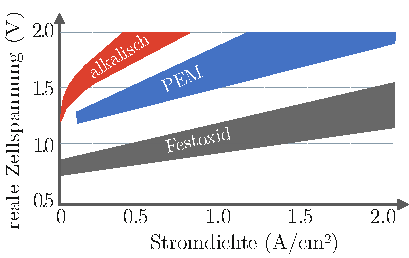
\includegraphics[scale=1]{Figures/PolarisationskurvenElektrolyseure}
		\caption{Mögliche Bereiche der Polarisationskurven verschiedener Elektrolyse-Technologien nach \cite{https://doi.org/10.1007/978-3-319-72459-1}}
\label{fig:PolarisationskurveElektrolyseure}	
\end{figure}

Des weiteren lässt sich mithilfe der Polarisationskurve auch die Abhängigkeit des Wirkungsgrades von der Stromdichte ableiten: Die elektrische Leistung einer Zelle ($P_el$) lässt sich aus der Stromdichte ($i$), der aktiven Fläche ($A_zelle$) und der realen Zellspannung errechnen. Das Faradaysche Gesetzt liefert einen direkten Zusammenhang zwischen de Elektronenfluss und dem Stoffmenge an produziertem Wasserstoff ($\dot{N}_{H_2O}$).
\begin{align}
	P_{el}(i) = U_{real}(i)\cdot i A_{zelle}\\
	\dot{N}_{H_2O} = \frac{i A_{zelle}}{nF}
\end{align}
Der Wirkungsgrad ($\eta$) einer Zelle, bezogen auf den unteren Heizwert ($H_u$) von Wasserstoff wird damit durch folgenden Ausdruck beschrieben:
\begin{align}
	\eta = \frac{H_u \cdot\dot{N_{H_2O}}}{P_{el}} = \frac{H_u}{U_{real}(i)\cdot{nF}}
\end{align}
Somit zeigt sich, dass es zur Steigerung der Effizienz erstrebenswert ist, den Elektrolyseur bei einer niedrigen Spannungen bzw. einer niedrigen Stromdichte zu betreiben [\cite{A semiempirical study of the temperature dependence of the anode charge transfer coefficient of a 6 kW PEM electrolyzer}]. Allerdings bleibt zu bedenken, dass dadurch auch der Produktgasstrom verringert wird, weshalb ein Kompromiss zwischen Wirkungsgrad und einer größeren aktive Zellflächen, und damit verbunden höheren Investitionskosten und größerem Bauraum, zu finden ist.\\
Weiterhin stellt die Gasreinheit der Produktströme eine untere Betriebsgrenze für die Stromdichte dar. Aufgrund von Diffusion durch Membran (bei Alkalischer und PEM-Elektrolyse) bzw. Elektrolyt(bei SO-Elektrolyse) kommt es zu einer Mischung von Sauerstoff und Wasserstoff. Da beide Produktgase bei einer Verunreinigung von $4$ bis $96$ Volumen-\% explosive Mischungen bilden können, wird üblicherweise bei 2 Volumen-\% Verunreinigung ein Notstop des gesamten Elektrolyseur-Systems eingeleitet.  Dabei lassen sich physikalisch zwei Abhängigkeiten erklären:\\ 
Einerseits nimmt die Verunreinigung der Produktgase bei hohem Druck zu, da dann auch der für die Diffusion maßgebliche Konzentrationsgradient eines Gases in der Membran/dem Elektrolyt steigt.\\
Andererseits sinkt die Verunreinigung bei steigender Stromstärke, weil die produzierte Stoffmenge mit der Stromdichte linear ansteigt, der Diffusionsstrom aber wegen gleichbleibender Konzentrationsverläufe  nahezu konstant ist. Somit ist wird die Verunreinigung bei einer höheren Stromdichte stärker verdünnt [\cite{Alkaline Water Electrolysis Powered by Renewable Energy: A Review}].
\cite{High-pressure PEM water electrolysis and corresponding safety
issues} gibt an, dass die Verunreinigung der Produktgase insbesondere durch die Rekombination von Wasserstoff und Sauerstoff verringert werden kann. Eine technische Lösung ist beispielsweise das Einbringen von Platin bei Anode und Kathode. Somit kann durch bestimmte Maßnahmen der Betriebsbereich in Richtung niedrigerer Stromstärken erweitert werden.
%7 Seiten
\subsection{Brennstoffzelle}
Funktionsprinzip und Gleichungen der Brennstoffzelle
%3 Seiten??